\documentclass{article}
\usepackage[utf8]{inputenc}
\usepackage[T1]{fontenc}
\usepackage{graphicx}
\usepackage{hyperref}
\usepackage{geometry}
\geometry{margin=1in}

\title{SWI  248 SYD}
\date{Encyclopaedia Britannica (1771)}

\begin{document}
\maketitle

\section*{Historical source}
\textbf{Entry ID:} \texttt{entry-swi-248-syd-251} \\
\textbf{Volume ID:} 191679021 \\
\textbf{Character Count:} 3905

\subsection*{Extracted Text}
parts of the country that border on Italy or France, a cor-
tune French in Italian prevails. The two predominant se
regions are Calvinia and Sprayer. Of the former we are the
centons of Zurich and Berne, the town of St Galli, Geneva, Malhland’s and Mali, the principality of Nuofstadt, the
gener part of Buli, Schaffaudins, the country of the Gris
foas, the Thurgun, Toggenburg, Glaris, and the Rhine valley. I
the Services of Appeares with a small part of Sabo
shum, and lines places at the countries of Canada and Dur-
gans. The refl of the Swifs cantons, allies and dependents
are People for the dejection of words there is an univer-
fly at Bali, and scadoniais e zurücke, Beren, Lauderians and
Geneva, heldes gymnaliums and échelle illulites, both in the
Ripih and Decerbat cantons. There are also focéeste a-
mong them for the improvement of the German language
and the fiecences.

Switect- land.

The principal manufactures are fluff and toboyen, lines
of several forks, here, threads, folk, and worried fleidings,
neckoloths cotton fluffy, gloves, handkerchiefs, flisks of fever-
alters, cold and five brecords, a variety of woollen manu-
factures, lats, paper, leather of alflor, earthous wers, por-
edain, toys, watches, clocks, and other hardwares, \&c.
The trade of Switzerland is greatly promoted by many na-
vigable lakes and rivers. In form of the above manufacture,
and in dieels, butter, fleep, horfes, black cattle, hides, and
flans, the experts are considerable and as the imports of the
chiely granulated fish, with some Americans at Arielie goods,
there is probably a large balance in their favour. In fome
parts of Switzerland dests is obtained by fampiary law.

The public revenues are in general very incredible,
arising chiefly from the usual regular, appropriated every
where to the foreignee, the domestic, and they gradually,
voluntary contributions, the fate of falls, and a land tax; in
the Protected cantons, from the church lands alto that were
fored at the Reforation. Except in Zuricha, Bern, Bull,
and Schaffaudines, where the people are more industrations,
have a greater trade and are richer than in the others, shall
use it was.

The cantons never keep any binding croops, except for a
few garrimsy but their militits is reckoned to be the belt
regulations of any in Europe. Every male from 16 to 05 i
enrolled, and about one third of them regimented. They
mult all provide therefore with arms, clothing, and word
traumatic, and appear on the dateted day for exercise, and the
feronal cantons and dirithate mult he furished with a futitic
ent train of artilities, and all its other implementos of war.
The Switect of the fereral cantons are allowed to engage
in the ferice of fuch foreign princes and flatters are in ali-
ance with their eastern or with whom they have made a pre-
vous agreement. Such latter, paying an annual fidelity to the
reflective cantons, are allowed to make lexies. Every man
enulis voluntarily, and for what number of years he pleties'
as the expiration of which he is at liberty to return
home. A great may thus always returning from foreign
ferivs. Switzerland is never unproceeded with, able and see
preferred effect and address. With and see
reproduced effect and utilities in their character, they are a brave, loose, hoofst, hoofntable, hardy people;
very true to their engagements, friendly and humane. In
fany, there is not a people in Europe who want much che
valdier is better. In their periods they are generally tall,
roahik, and wellness is, but their complications are now of
the belt, and clubs that live in the neighborhood of the
mountains are fidjekt to wens. The women are fail to be
generally headline and well-disped, reliable and modelly
transk, city, and vascade the conversation. Few of the
peelants are miribably poor; many of them are rich, efpec-
ically in the Protifiant cantons, and that of Berne in partic-
ular.

\subsection*{Matched Wikipedia Article}
\textbf{Title:} SWI \\
\textbf{Page ID:} 1287439 \\
\textbf{Revision ID:} 1320812045 \\
\textbf{URL:} \url{https://en.wikipedia.org/wiki/SWI}


\section*{Source record}
\begin{itemize}
\item \textbf{Dataset:} \texttt{NationalLibraryOfScotland/encyclopaedia\_britannica\_illustrated}
\item \textbf{Dataset Revision:} \texttt{309f765b1ecc83e0a7f7762e44b4a927a7555443}
\item \textbf{Page ID:} \texttt{britannica:309f765b1ecc83e0a7f7762e44b4a927a7555443:train:251} \\
  \textbf{Filename:} \texttt{page-0251-69952e7c4a0f.jpg} \\
  \textbf{Row Index:} 251 \\
  \textbf{SHA256:} \texttt{69952e7c4a0f4026...}
\end{itemize}

\begin{figure}[h]
\centering
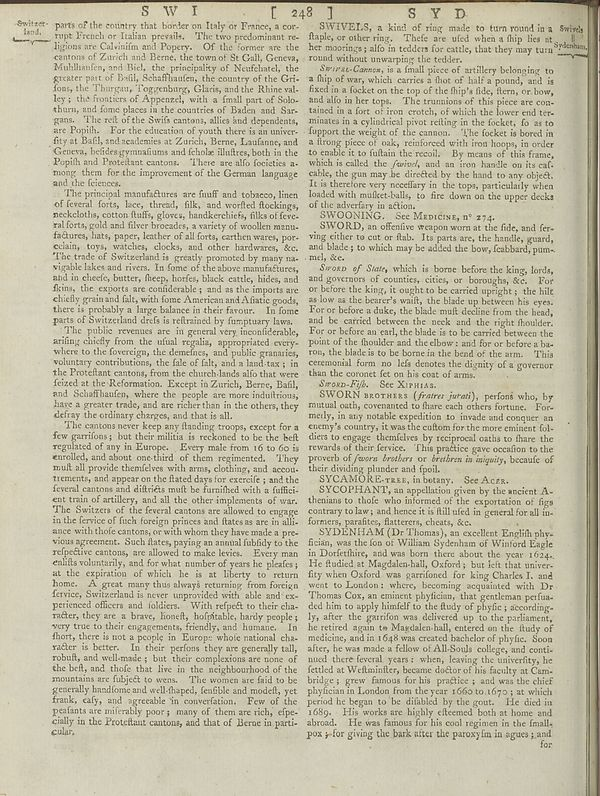
\includegraphics[width=0.85\textwidth]{../scans/page-0251-69952e7c4a0f.jpg}
\caption*{Source scan: \texttt{page-0251-69952e7c4a0f.jpg}}
\end{figure}

\end{document}
